\documentclass[11pt]{article}
\usepackage{geometry,marginnote} % Pour passer au format A4
\geometry{hmargin=1cm, vmargin=1cm} % 

% Page et encodage
\usepackage[T1]{fontenc} % Use 8-bit encoding that has 256 glyphs
\usepackage[english,french]{babel} % Français et anglais
\usepackage[utf8]{inputenc} 

\usepackage{lmodern,numprint}
\setlength\parindent{0pt}

% Graphiques
\usepackage{graphicx,float,grffile,units}
\usepackage{tikz,pst-eucl,pst-plot,pstricks,pst-node,pstricks-add,pst-fun,pgfplots} 

% Maths et divers
\usepackage{amsmath,amsfonts,amssymb,amsthm,verbatim}
\usepackage{multicol,enumitem,url,eurosym,gensymb,tabularx}

\DeclareUnicodeCharacter{20AC}{\euro}



% Sections
\usepackage{sectsty} % Allows customizing section commands
\allsectionsfont{\centering \normalfont\scshape}

% Tête et pied de page
\usepackage{fancyhdr} \pagestyle{fancyplain} \fancyhead{} \fancyfoot{}

\renewcommand{\headrulewidth}{0pt} % Remove header underlines
\renewcommand{\footrulewidth}{0pt} % Remove footer underlines

\newcommand{\horrule}[1]{\rule{\linewidth}{#1}} % Create horizontal rule command with 1 argument of height

\newcommand{\Pointilles}[1][3]{%
  \multido{}{#1}{\makebox[\linewidth]{\dotfill}\\[\parskip]
}}

\newtheorem{Definition}{Définition}

\usepackage{siunitx}
\sisetup{
    detect-all,
    output-decimal-marker={,},
    group-minimum-digits = 3,
    group-separator={~},
    number-unit-separator={~},
    inter-unit-product={~}
}

\setlength{\columnseprule}{1pt}

\begin{document}

\horrule{2px}
\section*{Chapitre 3 - Triangles}
\horrule{2px}

\begin{Definition}{Le triangle}\\
  Un triangle est une figure géométrique qui a : 
  \begin{itemize}
    \item 3 sommets
    \item 3 angles
    \item 3 côtés
  \end{itemize}
\end{Definition}

Existe-t-il des conditions pour construire un triangle à partir de ces trois définitions.

\section*{3 sommets ?}

\textbf{Il faut que les sommets ne soient ni confondus ni alignés.}

\section*{3 angles ?}

\begin{Definition}{La somme des angles dans un triangle}\\
  \textbf{La somme des angles dans un triangle fait 180°.}
\end{Definition}


\textbf{Méthode exercice angles :}

\begin{itemize}
  \item On cite la définition : \textbf{La somme des angles dans un triangle fait 180°.}
  \item \textbf{Modéliser : } On transforme notre énoncé géométrique en un énoncé de type mathématiques.
  \item \textbf{Calculer : } On transforme notre énoncé mathématiques en un calcul. 
\end{itemize}

\horrule{1px}
\textbf{Ex1 : Calculer les angles manquants.}
\textit{Ex1' : Il est possible de transformer cet exercice en mettant tous les angles dans le triangle et en demandant si on peut le construire.}

\begin{figure}[H]
  \centering
  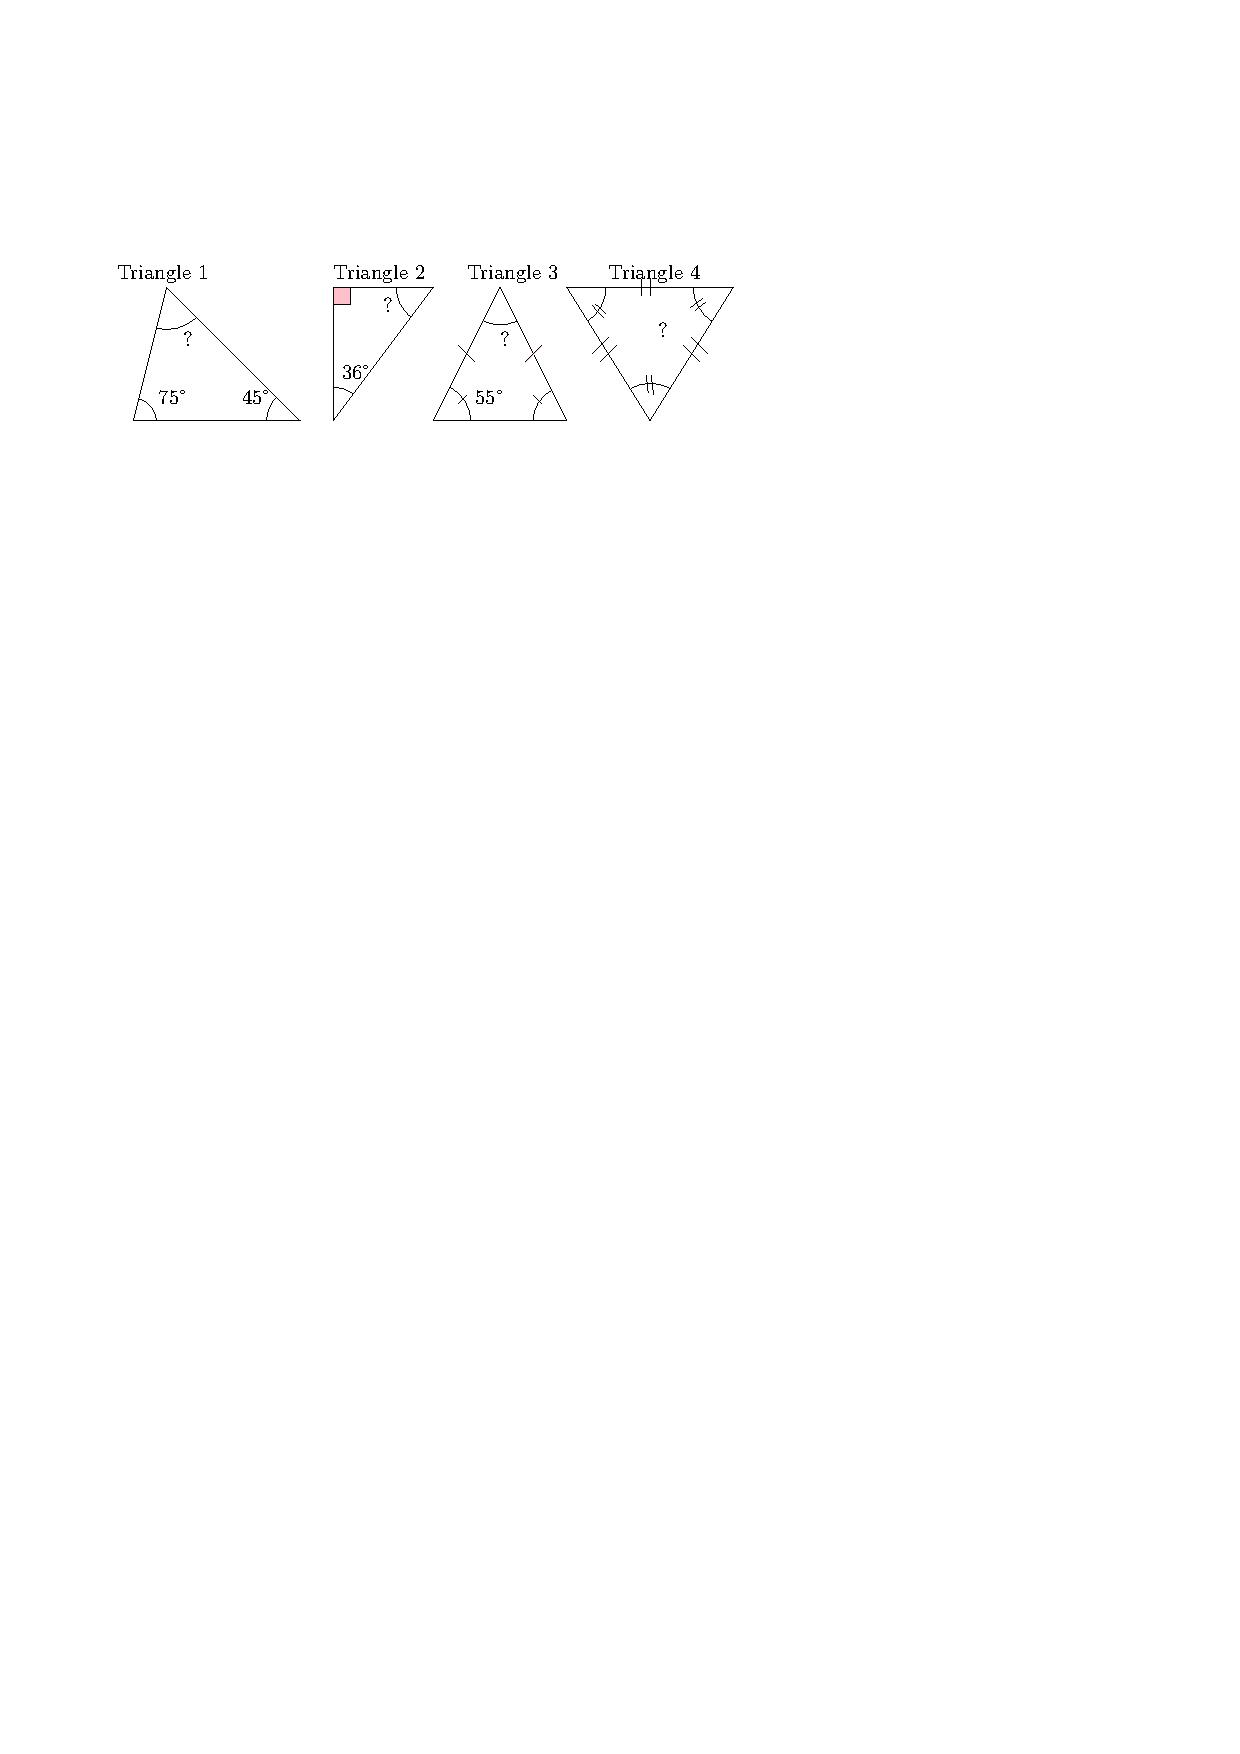
\includegraphics[width=0.7\linewidth]{5x3-triangles/m1-exo.pdf}
\end{figure}

\begin{multicols}{2}

  \textsc{Triangle 1}
  \begin{itemize}[label={$\bullet$}]
    \item \textbf{Modéliser : } $45 + 75 + \dots = 180 \degree$
    \item \textbf{Calculer : } $180 - (45 + 75) = 60\degree$
  \end{itemize}

  \textsc{Triangle 2}
  \begin{itemize}[label={$\bullet$}]
    \item \textbf{Modéliser : } $90 + 36 + \dots = 180\degree$
    \item \textbf{Calculer : } $180 - (90 + 36) = 54\degree$
  \end{itemize}
  \columnbreak

  \textsc{Triangle 3}
  \begin{itemize}[label={$\bullet$}]
     \item \textbf{Modéliser : } $55 \times 2 + \dots = 180\degree$
     \item \textbf{Calculer : } $180 - 55 \times 2 = 70\degree$
  \end{itemize}

  \textsc{Triangle 4}
  \begin{itemize}[label={$\bullet$}]
    \item \textbf{Modéliser : } $3 \times \dots = 180\degree$
    \item \textbf{Calculer : } $180 \div 3 = 60\degree$
  \end{itemize}

\end{multicols}

Des rappels en vrac : 

\begin{itemize}
  \item Un angle droit mesure 90°.
  \item Un angle tour complet mesure 360°.
  \item Un triangle isocèle a 2 côtés de même longueur et deux angles de même mesure.
  \item Un triangle équilatéral a 3 côtés de même longueur et trois angles de même mesure. (60°)
\end{itemize}

\section*{3 longueurs ?}

\begin{Definition}{L'inégalité triangulaire}\\
  \textbf{Le plus grand côté d'un triangle doit être plus petit que la somme des autres.}
\end{Definition}

\textbf{Méthode exercice longueurs :}

\begin{itemize}
  \item On cite la définition : \textbf{Le plus grand côté d'un triangle doit être plus petit que la somme des autres.}
  \item On trouve le plus grand côté.
  \item On calcule la somme des deux autres.
  \item On compare.
  \item On conclut. 
\end{itemize}

\horrule{1px}
\textbf{Ex2 : Peut-on construire le triangle ?}

1. On cherche à construire un triangle ABC tel que  AB = 6cm, BC = 12cm et AC = 4cm. 

\begin{itemize}[label={$\bullet$}]
  \item Le plus grand côté est : $BC = 12cm$
  \item $AB + AC = 6 + 4$ \newline
        $AB + AC = 10cm$ 
  \item 10 < 12 donc BC < AB + AC
  \item Le triangle ne peut pas être construit.
\end{itemize}

2. On cherche à construire un triangle RST tel que  RS = 16cm, RT = 12cm et ST = 24cm. 

\begin{itemize}[label={$\bullet$}]
  \item Le plus grand côté est : $ST = 24cm$
  \item $RS + RT = 16 + 12$ \newline
        $RS + RT = 28cm$ 
  \item 28 > 24 donc ST > RS + RT
  \item Le triangle peut être construit.
\end{itemize}


\end{document}
